\documentclass{classes/fiboReport}

\begin{document}

\Modifydate{21/04/2018}
\subject{FRA501 Principles of Model-based Design in Robotics}
\title{Quadrotor Dynamic Modelling}
\subtitle{การโมเดลระบบของอากาศยานสี่ใบพัด}
\academicyear{2560}
\coverimage{cover.jpg}
\covertext{
	\begin{tabular}{ l l }
		{นายจุฬภัทร จิรชัย} & {57340500013} \\  
		{นายเจตนันท์ หอมจันทนากุล} & {57340500015} \\
		{นายวุฒิภัทร โชคอนันตทรัพย์} & {57340500067}  
	\end{tabular}
}
\pagecolor{tudelft-cyan}
\advisor{อาจารย์ธนัชชา ชูพจน์เจริญ}

\maketitle
\frontmatter
% ************************** Thesis Abstract **********************************
\begin{abstract}

\end{abstract}
\tableofcontents
% \listoffigures
% \listoftables
% % ***************************** Thesis Symbols ********************************
\begin{symbols}
    \noindent
    \begin{tabular*}{\textwidth}{@{}p{0.18\textwidth}p{0.8\textwidth}@{}}
        {$\theta$} & {เซต้า} \\
        {$d$} & {distance} \\
        {kg} & {Kilogram} \\
        {m$^{2}$} & {Square Metre} \\
    \end{tabular*}
\end{symbols}
% % ************************** Thesis Abbreviations **************************
\begin{abbreviations}
    \noindent
    \begin{tabular*}{\textwidth}{@{}p{0.18\textwidth}p{0.8\textwidth}@{}}
        {UTHAI} & {Universal Template for Humanoid Algorithm Interface} \\
        {ROS} & {Robot Operating System} \\
        {IMU} & {Inertial Measurement Unit} \\
        {DoF} & {Degree of Freedom} \\
        {CoM} & {Center of Mass} \\
        {ZMP} & {Zero Moment Point} \\
        {PLA} & {Polylactic acid} \\
        {ABS} & {Acrylonitrile butadiene styrene} \\
        {KMUTT} & {King Mongkut's University of Technology Thonburi} \\
        {Liews} & {วุฒิภัทร โชคอนันตทรัพย์} \\
        {$\theta$} & {เซต้า}
    \end{tabular*}
\end{abbreviations}





% \begin{figure}[ht]
% 	\centering
% 	\includegraphics[width=0.5\textwidth]{Images/maplestory_1.jpg}
% 	\caption{Example of a parametric plot ($\sin (x), \cos(x), x$)}
% \end{figure}
% \begin{Verbatim}
% 	% dskfaosdlfk
% 	#include <stdio.h>
% 	int main()
% 	{
% 		printf("Hello World");
% 		return 0;
% 	}
% \end{Verbatim}
\mainmatter
\chapter{Introduction}
อากาศยานสี่ใบพัด (quadrotor) คือเฮลิคอปเตอร์หลายใบพัด (multi-helicopter) ที่มีลักษณะใบพัดเรียงตัวกันเป็นรูปสี่เหลื่ยมมุมฉาก
หรือเป็นรูปทรงที่มีความสมมาตร เพื่อใช้ในการพยุงพาหนะและควบคุมทิศทางได้อย่างเป็นอิสระมากขึ้นเมื่อเทียบกับเฮลิคอปเตอร์ทั่วไป
โดยในปัจจุบัน อากาศยานสี่ใบพัดได้ถูกนำมาประยุกต์ใช้งานในหลากหลายรูปแบบ ยกตัวอย่างเช่น ด้านเกษตรกรรม(ใช้ในการฉีดยาป้องกันศัตรูพืชหรือตรวจสอบผลิตผลเพื่อช่วยเกษตรกร)
ด้านอุตสาหรรม(ใช้สำรวจรอยรั่วที่หลังคาของโรงงาน บ้านเรือน) ด้านการทหาร(ใช้ในการสำรวจพื้นที่ ตรวจดูที่ตั้งของศัตรู) ด้านกู้ภัยฉุกเฉิน(ใช้ในการหาพื้นที่ประสบภัย ไฟไหม้)
ด้านการบันเทิง(ใช้แปรอักษรเป็นรูปภาพและเคลื่อนที่ในรูปแบบต่างๆ) เป็นต้น ซึ่งจะเห็นได้ว่าอากาศยานสี่ใบพัดนั้นสามารถนำไปใช้ได้ในหลากหลายทาง
แต่ด้วยจำนวนของใบพัดที่มีมาก ทำให้ระบบมีกลไกและกระบวนการในการควบคุมที่มีความซับซ้อนมากขึ้น
ทางคณะผู้จัดทำจึงสนใจที่จะทำโครงงานเกี่ยวกับอากาศยานสี่ใบพัด เพื่อศึกษาพลศาสตร์และออกแบบระบบควบคุม รวมไปถึงการจำลองการเคลื่อนที่ของอากาศยาน
โดยทำผ่านโปรแกรมจำลอง และนำความรู้ทั้งหมดไปใช้ในการพัฒนาการทำงานของอากาศยานสี่ใบพัดต่อไปในอนาคต

\chapter{System Description}
\section{Quadroter mathematical model}
\subsection{Preliminar notions}
โดรนเป็นอากาศยานชนิดหนึงที่มีมอเตอร์เป็นตัวขับเคลื่อนอยู่ 4 ตัว มีบอร์ดควบคุมและสั่งการอยู่ตรงกลางระหว่างมอเตอร์ทั้งสี่
ก่อนจะหาสมการคณิตศาสตร์ของโดรนนั้น จะต้องเริ่มจากรู้จักเฟรมอ้างอิงก่อน เฟรมอ้างอิงนี้จะช่วยบอกได้ว่าตัวโดรนนั้นอยู่ที่ตำแหน่งไหน
เอียงอย่างไรอยู่ เฟรมอ้างอิงของโดรนนั้นใช้เพียง 2 เฟรมด้วยกัน คือเฟรมที่อยู่กับที่ไม่ขยับไปไหน และเฟรมที่เคลื่อนที่ไปมา
เฟรมแรกคือเฟรมที่อยู่กับที่นั้นมีชื่อว่า \quotes{Inertial frame} เฟรมนี้เอาไว้สำหรับใช้ในการอ้างอิงพื้นโลก
โดยที่ทิศทางของแรงโน้มถ่วง (gravity) จะมีทิศทางไปทางแกน -Z ของ \quotes{Inertial frame}
ส่วนเฟรมอีกอันคือ \quotes{Body frame} เฟรมนี้เอาไว้ใช้สำหรับในการบอกตำแหน่งและการเอียงของตัวโดรน
โดยการบอกนั้นจะบอกเทียบกับ \quotes{Inertial frame} การตั้งเฟรมนี้นั้นจะให้แกน +Z ชี้ไปตามทิศของมอเตอร์ทั้งสี่ ดังรูปที่ \ref{fig:quadroter_coordinates}

\begin{figure}[ht]
	\centering
	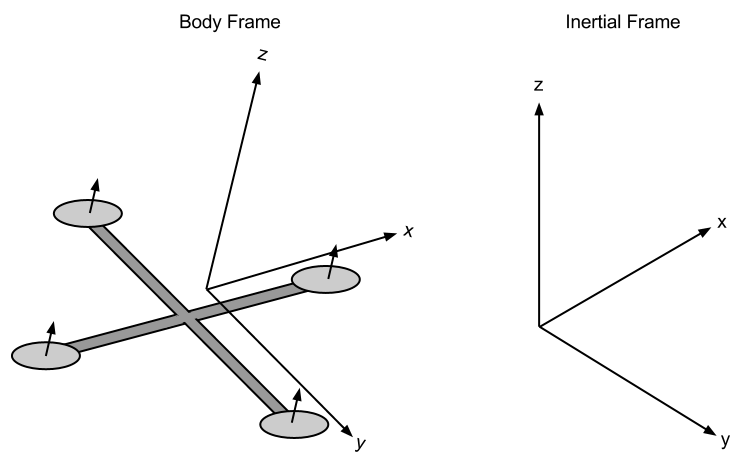
\includegraphics[width=0.6\textwidth]{images/Quadcopter_Coordinates.png}
	\caption{เฟรมอ้างอิงของโดรน}
	\label{fig:quadroter_coordinates}
\end{figure}

การควบคุมตำแหน่งและท่าทางของโดรนนั้น เราสามารถควบคุมได้โดยการสั่งให้มอเตอร์ทั้งสี่ตัวมีความเร็วที่แตกต่างกัน
เมื่อมอเตอร์หมุนด้วยความเร็วไม่เท่ากันจะทำให้เกิดแรงและโมเมนต์ขึ้นที่ตัวโดรน แรงยกนั้นจะเกิดขึ้นจากการหมุนมอเตอร์ทั้งหมด
ส่วนการเอียง Pitch (หมุนรอบแกน Y ของ Body frame), Roll (หมุนรอบแกน X ของ Body frame)
จะเกิดจากความแตกต่างระหว่างแรงยกของมอเตอร์ทั้งสี่ตัว แรงโน้มถ่วงของโลก และ Yaw (หมุนรอบแกน Z ของ Body frame)
เกิดจากการที่มอเตอร์หมุนด้วยความเร็วที่ไม่สมดุลกัน โดรนจะไม่หมุน Yaw หากมีมอเตอร์หมุนไปในทิศทางตรงกันข้ามกัน
ดังนั้นทำให้เราสามารถแบ่งใบพัดของโดรนออกเป็น 2 กลุ่ม แต่ละกลุ่มจะมีทิศทางการหมุนตรงข้ามกันและอยู่ฝั่งตรงกันข้ามกัน

\begin{itemize}
	\setlength\itemsep{-0.3em}
	\item ใบพัด หน้า และ หลัง (เลข 2 และเลข 4 ในรูปที่ \ref{fig:quadroter_rotordirection} ) จะหมุนทวนเข็มนาฬิกา CCW
	\item ใบพัด ซ้าย และ ขวา (เลข 1 และเลข 3 ในรูปที่ \ref{fig:quadroter_rotordirection} ) จะหมุนตามเข็มนาฬิกา CW
\end{itemize}

\begin{figure}[ht]
	\centering
	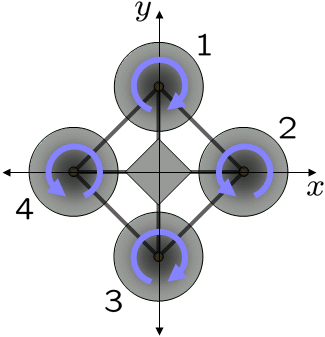
\includegraphics[width=0.4\textwidth]{images/Quadcopter_RotorDirection.png}
	\caption{ทิศทางการหมุนของแต่ละใบพัด}
	\label{fig:quadroter_rotordirection}
\end{figure}

การเคลื่อนที่ในปริภูมิของโดรนนั้นเราสามารถแบ่งได้ออกเป็น 2 ส่วนคือ การเคลื่อนที่ตามแนวแกน
และการเคลื่อนที่หมุนรอบแกน ในการอธิบายการเคลื่อนที่ของโดรนนั้น หากนับองศาอิสระจะได้ทั้งหมดเป็น 6 องศาอิสระ
โดย 6 องศาอิสระนี้คือ การเคลื่อนที่ตามแนวแกน 3 แกน (X Y Z) และการเคลื่อนที่หมุนรอบแกน (Roll Pitch Yaw)
การควบคุมการเคลื่อนที่ใน 6 องศาอิสระนั้นสามารถทำได้โดยปรับความเร็วการหมุนของมอเตอร์ให้มีความแตกต่างกัน
การเคลื่อนที่ไปข้างหน้า ถอยหลัง ไปด้านข้าง ขึ้นลง หมุนรอบ Roll Pitch Yaw,
ที่โดรนสามารถหมุนรอบแกน Yaw ได้นั้นเกิดจากทอร์คของมอเตอร์ทั้งสี่ ผลรวมของทอร์คจะส่งผลต่อความเร็วในการหมุนรอบแกน Yaw
หากมอเตอร์ทุกตัวหมุนด้วยความเร็วเท่ากัน ผลรวมทอร์คจะมีค่าเท่ากับศูนย์ทำให้โดรนไม่หมุน แต่ถ้ามอเตอร์หมุนด้วยความเร็วไม่เท่ากัน
จะทำให้ผลรวมทอร์คมีค่าไม่เท่ากับศูนย์จะส่งผลให้โดรนเกิดการหมุนรอบแกน Yaw ได้
ถ้ามอเตอร์ทุกตัวหมุนด้วยความเร็วเพิ่มขึ้นหรือลดลงพร้อมกันจะทำให้โดรนเคลื่อนที่ขึ้นหรือลงตามแนวดิ่ง
และด้วยการที่เรามี 4 Inputs แต่มี 6 Outputs นั้นทำให้การควบคุมโดรนเป็นแบบ Underactuated ซึ่งมีความซับซ้อนพอสมควร
เพื่อที่จะคอนโทรลโดรนได้นั้น ให้สมมุติว่าตัวโดรนเป็นวัตถุชิ้นเดียว (Rigid body) โครงสร้างมีความสมมาตร (Symmetric)
ความเร็วของแต่ละมอเตอร์ จะทำให้ใบพัดมีแรงยก เราสามารถบอกลักษณะการเคลื่อนที่ของโดรนได้ ดังรูปที่ \ref{fig:quadroter_movement}

\begin{figure}[ht]
	\centering
	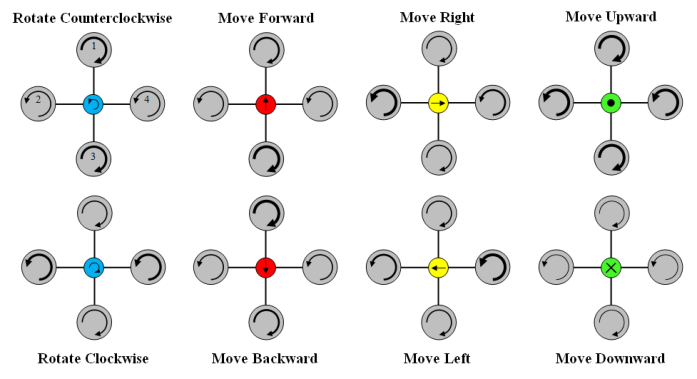
\includegraphics[width=0.95\textwidth]{images/Quadcopter_Movement.png}
	\caption{ทิศทางการเคลื่อนที่ของโดรนเมื่อมอเตอร์หมุนด้วยความเร็วต่างๆ}
	\label{fig:quadroter_movement}
\end{figure}
\clearpage
\subsection{Euler angles}
มุมออยเลอร์เป็นมุม 3 มุมที่คิดโดย Leonhard Euler เพื่อที่จะเอาไว้ใช้อธิบายการเอียงของวัตถุในปริภูมิ
ใช้ตัวแปรเพียงแค่ 3 ตัวเท่านั้น การบอกมุมออยเลอร์สามารถบอกได้หลายวิธี ในที่นี้เราใช้ ZYX Euler angles
ในการอธิบายมุมเอียงของเฟรมอ้างอิงที่เราสนใจเทียบกับเฟรมอ้างอิงเฟรมอื่น มุมออยเลอร์เกิดจากการหมุนเฟรมรอบแกนสามแกน
มาหมุนเรียงต่อกัน ต่อไปจะเป็นการรวมแมทริกการหมุนสามแกนเข้าด้วยกัน

\begin{equation}
	{R_{x}(\phi) = \begin{bmatrix}
		1 & 0 & 0 \\
		0 & c(\phi) & -s(\phi) \\
		0 & s(\phi) & c(\phi)
		\end{bmatrix}}
	\label{equ:rotation_matrix_x}
\end{equation}

\begin{equation}
	{R_{y}(\theta) = \begin{bmatrix}
		c(\theta) & 0 & s(\theta) \\
		0 & 1 & 0 \\
		-s(\theta) & 0 & c(\theta)
		\end{bmatrix}}
	\label{equ:rotation_matrix_y}
\end{equation}

\begin{equation}
	{R_{z}(\psi) = \begin{bmatrix}
		c(\psi) & -s(\psi) & 0 \\
		s(\psi) & c(\psi) & 0 \\
		0 & 0 & 1 \\
		\end{bmatrix}}
	\label{equ:rotation_matrix_z}
\end{equation}

โดยที่ $c(\phi) = cos(\phi)$, $s(\phi) = sin(\phi)$, $c(\theta) = cos(\theta)$, $s(\theta) = sin(\theta)$, $c(\psi) = cos(\psi)$, $s(\psi) = sin(\psi)$
จากแมทริกการหมุนแสดงให้เห็นว่า \quotes{Inertial frame} และ \quotes{ฺBody frame}
มีความสัมพันธ์กันเป็นแมทริกการหมุนคือ $R_{zyx}(\phi,\theta,\psi)$
\begin{equation}
	\begin{array}{c}
		{R_{zyx}(\phi,\theta,\psi) = R_{z}(\psi)R_{y}(\theta)R_{x}(\phi)}\\
		{= \begin{bmatrix}
		c(\theta)c(\psi) & s(\phi)s(\theta)c(\psi)-c(\phi)s(\psi) & c(\phi)s(\theta)c(\psi)+s(\phi)s(\psi) \\
		c(\theta)s(\psi) & s(\phi)s(\theta)c(\psi)+c(\phi)s(\psi) & c(\phi)s(\theta)c(\psi)-s(\phi)c(\psi) \\
		-s(\theta)       & s(\phi)c(\theta)                       & c(\phi)c(\theta)                       \\
		\end{bmatrix}}
		\label{equ:rotation_matrix_zyx}
	\end{array}
\end{equation}

แมทริกจากสมการที่ \ref{equ:rotation_matrix_zyx} เป็นแมทริกที่อธิบายถึงการหมุนจาก \quotes{ฺBody frame} ไปยัง \quotes{Inertial frame}
ดังรูปที่ \ref{fig:quadroter_eulerangles}
\begin{figure}[htbp]
	\centering
	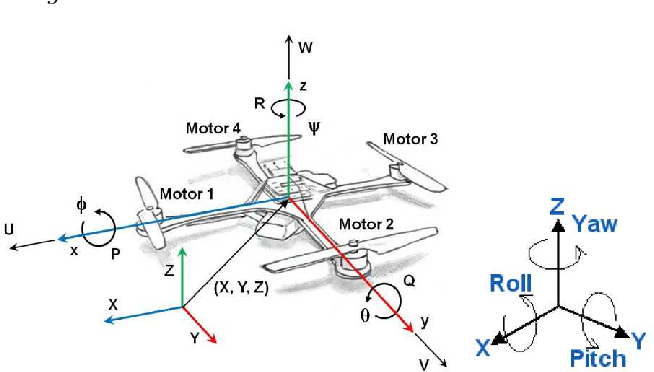
\includegraphics[width=0.65\textwidth]{images/Quadcopter_EulerAngles.png}
	\caption{ภาพแสดงการบอกแมทริกการหมุนของ Body frame}
	\label{fig:quadroter_eulerangles}
\end{figure}
\clearpage
\subsection{Qaudroter mathematical model}
ในส่วนนี้จะเป็นการอธิบายสมการการเคลื่อนที่ของโดรน โดยใช้สมการของ Newton และ Euler มาช่วยในการอธิบายพลวัต (Dynamics) ของโดรน
เพื่อใช้ทำแบบจำลอง (Simulating) และควบคุม (Controlling) ท่าทางของโดรนด้วย
เริ่มจากให้ $[\begin{matrix}x & y & z & \phi & \theta & \psi \end{matrix}]^T$ เป็นเวกเตอร์ที่บอกตำแหน่งและมุม (linear/angular position)
ของโดรนโดยเทียบจากเฟรมโลก (Inertial frame) และ $[\begin{matrix}u & v & w & p & q & r\end{matrix}]^T$ เป็นเวกเตอร์ที่บอกความเร็วเชิงเส้นและความเร็วเชิงมุม
(linear/angular velocity) ของโดนโดยเทียบจากเฟรมโดรน (Body frame) พลวัตของโดรนจะเปิดจากเฟรมอ้างอิงสองเฟรมนี้มีความสัมพันธ์กัน

\begin{equation}
	\begin{array}{c}
		{\nu = R\nu_{B}}               \\
		{\omega = T\omega_{B}}         
		\label{equ:equation_of_motion} 
	\end{array}
\end{equation}

โดยที่ $\nu = [\begin{matrix}\dot{x} & \dot{y} & \dot{z} \end{matrix}]^T$, $\omega = [\begin{matrix}\dot\phi & \dot\theta & \dot\psi \end{matrix}]^T$,
$\nu_{B} = [\begin{matrix}u & v & w \end{matrix}]^T$, $\omega_{B} = [\begin{matrix}p & q & r \end{matrix}]^T$ และ $T$
เป็นแมทริกการแปลงมุมการหมุน (angular transformation)
\begin{equation}
	{T = \begin{bmatrix}
		1 & s(\phi)t(\theta) & c(\phi)t(\theta) \\
		0 & c(\phi) & -s(\phi) \\
		0 & \dfrac{s(\phi)}{c(\theta)}  & \dfrac{c(\phi)}{c(\theta)} \\
		\end{bmatrix}}
	\label{equ:angular_transformation}
\end{equation}

โดยที่ $t(\theta) = tan(\theta)$ ดังนั้นเราจะได้สมการจลศาสตร์ (Kinematic model) ของโดรนเป็น
\begin{equation}
	{\begin{bmatrix}
		\dot{x}  \\
		\dot{y}  \\
		\dot{z} \\
		\dot{\phi} \\
		\dot{\theta} \\
		\dot{\psi} \\
		\end{bmatrix} = 
		\begin{bmatrix}
			w[s(\phi)s(\psi)+c(\phi)c(\psi)s(\theta)]-v[c(\phi)s(\psi)-c(\psi)s(\phi)s(\theta)]+u[c(\psi)c(\theta)] \\
			v[c(\phi)c(\psi)+s(\phi)s(\psi)s(\theta)]-w[c(\psi)s(\phi)-c(\phi)s(\psi)s(\theta)]+u[c(\theta)s(\psi)] \\
			w[c(\phi)c(\theta)]-u[s(\theta)]+v[c(\theta)s(\phi)]                                                    \\
			p+r[c(\phi)t(\theta)]+q[s(\phi)t(\theta)]                                                               \\
			q[c(\phi)]-r[s(\phi)]                                                                                   \\
			r\dfrac{c(\phi)}{c(\theta)}+q\dfrac{s(\phi)}{c(\theta)}                                                 \\
		\end{bmatrix}	}
	\label{equ:kinematic model}
\end{equation}

จากกฎของนิวตันระบุความสัมพันธ์ของแรงรวมที่กระทำต่อโดรนดังเมทริกซ์ต่อไปนี้

\begin{equation}
	{ m(\omega_B\wedge \nu_B+\dot{\nu_B})=\mathbf{f}_B}
	\label{equ:total force}
\end{equation}

โดย $m$ คือน้ำหนักของโดรน , $\wedge$ คือ cross product และ $\mathbf{f}_B=\begin{bmatrix}f_x & f_y & f_z \end{bmatrix}^T \in \mathbf{R}^3$ 
คือแรงรวม
\\ จากสมการออยเลอร์ ให้แรงบิดรวมที่ใช้กับโดรน เป็นไปดังนี้

\begin{equation}
	{
		I.\dot{\omega}_B+\omega_B\wedge(I.\omega_B)=\mathbf{m}_B
	}
	\label{equ:total force}
\end{equation}
\\
โดย $\mathbf{m}_B=\begin{bmatrix}m_x & m_y & m_z\end{bmatrix}^T \in \mathbf{R}^3$ เป็นแรงบิดรวม และ $I$ เป็นเมทริกซ์ของความเฉื่อย :
\begin{equation}
	{
		I = \begin{bmatrix}I_x & 0 & 0 \\
		0   & I_y & 0 \\
		0   & 0 & I_z \\
		\end{bmatrix} \wedge \mathbf{R}^{3\times3}
	}
	\label{equ:inertia matrix}
\end{equation}

ดังนั้น จะได้ dynamic model ของโดรนโดยอ้างอิง body frame ดังนี้
\begin{equation}
	{
		\begin{bmatrix}	f_x \\
			f_y \\
			f_z \\
			m_x \\
			m_y \\
			m_z \\   
		\end{bmatrix} = 
		\begin{bmatrix}	m(\dot{u}+qw-rv) \\
			m(\dot{v}-pw+ru)       \\
			m(\dot{w}+pv-qu)       \\
			\dot{p}I_x-qrI_y+qrI_z \\
			\dot{q}I_y+prI_x-prI_z \\
			\dot{r}I_z-pqI_x+pqI_y \\   
		\end{bmatrix}
	}
	\label{equ:dynamic model}
\end{equation}

ซึ่งระบบต่าง ๆ จะเป็นไปตามสมการข้างต้นเมื่อกำหนดให้จุด origin และ body frame ตรงกับจุดเซนทรอยด์และ principal axes ของโดรน

% https://www.kth.se/polopoly_fs/1.588039!/Thesis%20KTH%20-%20Francesco%20Sabatino.pdf
\section{Explicit MPC Control}
% https://www2.eecs.berkeley.edu/Pubs/TechRpts/2012/EECS-2012-241.pdf


\chapter{Simulation}

\chapter{Analysis/Discussion}
\chapter{Conclusion}


\nocite{*}
\bibliographystyle{plain}
\bibliography{pages/reference}
\addcontentsline{toc}{chapter}{เอกสารอ้างอิง}
\end{document}